\documentclass[varwidth,border=0pt]{standalone}

% Tikz packages
\usepackage{tikz}
\usetikzlibrary{%
  patterns, plotmarks, backgrounds, shapes, arrows, calc, trees, positioning,
  chains, shapes.geometric, decorations.pathreplacing,
  decorations.pathmorphing, shapes.arrows, decorations.markings, quotes,
  arrows.meta, spy, fit, matrix
}

% General image and colour support
\usepackage{graphicx}
\usepackage{xcolor}

% Captions and subcaptions
\usepackage{caption}
\usepackage[labelformat=parens]{subcaption}
\renewcommand\thesubfigure{\alph{subfigure})}

% Define main node type for networks
\tikzstyle{lnode} = [%
  circle,
  draw=black,
  minimum height=0.65cm,
  align=center,
  fill=none,
  text centered,
  inner sep=0.5pt,
  font=\tiny
]%

\begin{document}
  \begin{figure}
    \centering
    \begin{subfigure}[t]{0.5\textwidth}
      \caption{}
      \vspace*{-1.5em}
      \centering
      \scalebox{0.75}{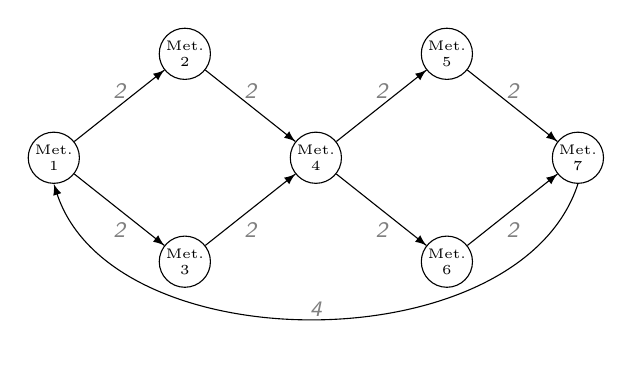
\begin{tikzpicture}[%
  >=latex,
  decoration={%
    markings,
    mark=at position 1.0 with {\arrow{>}}
  },
  every node/.style={%
    font=\sffamily\footnotesize\itshape,
    text=gray,
    text centered,
    align=center
  },
  frame/.style={draw=black,inner sep=2pt}
]

  % Nodes
  \node[lnode,text=black] (A1) {Met.\\1};
  \node[lnode,text=black,right=1.0cm of A1,yshift=1.32cm] (A2) {Met.\\2};
  \node[lnode,text=black,right=1.0cm of A1,yshift=-1.32cm] (A3) {Met.\\3};
  \node[lnode,text=black,right=1.0cm of A2,yshift=-1.32cm] (A4) {Met.\\4};
  \node[lnode,text=black,right=1.0cm of A4,yshift=1.32cm] (A5) {Met.\\5};
  \node[lnode,text=black,right=1.0cm of A4,yshift=-1.32cm] (A6) {Met.\\6};
  \node[lnode,text=black,right=1.0cm of A5,yshift=-1.32cm] (A7) {Met.\\7};

  % Intra-node edges
  \draw[postaction={decorate}] (A1) to node [above=0.1pt,yshift=-1pt] {2} (A2);
  \draw[postaction={decorate}] (A1) to node [below=0.1pt,yshift=-1pt] {2} (A3);
  \draw[postaction={decorate}] (A2) to node [above=0.1pt,yshift=-1pt] {2} (A4);
  \draw[postaction={decorate}] (A3) to node [below=0.1pt,yshift=-1pt] {2} (A4);
  \draw[postaction={decorate}] (A4) to node [above=0.1pt,yshift=-1pt] {2} (A5);
  \draw[postaction={decorate}] (A4) to node [below=0.1pt,yshift=-1pt] {2} (A6);
  \draw[postaction={decorate}] (A5) to node [above=0.1pt,yshift=-1pt] {2} (A7);
  \draw[postaction={decorate}] (A6) to node [below=0.1pt,yshift=-1pt] {2} (A7);

  % Boundary edges
  \draw[->, postaction={decorate}, bend left=72, distance=2.4cm] (A7.south) to node [above=0.1pt,yshift=-3pt] {4} (A1.south);

\end{tikzpicture}

}\\
      \vspace*{-1.5em}
      \scalebox{0.75}{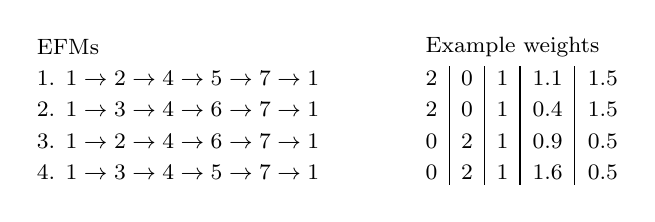
\begin{tikzpicture}[%
    >=latex,
    decoration={%
      markings,
      mark=at position 1.0 with {\arrow{>}}
    },
    every node/.style={%
      font=\sffamily\footnotesize\itshape,
      text=gray,
      text centered,
      align=center
    },
    frame/.style={draw=black,inner sep=2pt}
  ]

  \node[black, font=\rmfamily\footnotesize] (t1) {EFMs};
  \node[black, font=\rmfamily\footnotesize, below=0.4cm of t1.west, anchor=west]
    (t2)
    {1. $1 \rightarrow 2 \rightarrow 4 \rightarrow 5 \rightarrow 7 \rightarrow 1$};
  \node[black, font=\rmfamily\footnotesize, below=0.4cm of t2.west, anchor=west]
    (t3)
    {2. $1 \rightarrow 3 \rightarrow 4 \rightarrow 6 \rightarrow 7 \rightarrow 1$};
  \node[black, font=\rmfamily\footnotesize, below=0.4cm of t3.west, anchor=west]
    (t4)
    {3. $1 \rightarrow 2 \rightarrow 4 \rightarrow 6 \rightarrow 7 \rightarrow 1$};
  \node[black, font=\rmfamily\footnotesize, below=0.4cm of t4.west, anchor=west]
    (t5)
    {4. $1 \rightarrow 3 \rightarrow 4 \rightarrow 5 \rightarrow 7 \rightarrow 1$};
  \node[black, font=\rmfamily\footnotesize, right=3.9cm of t1] (u1) {Example weights\textcolor{white}{ss}};
  \node[black, font=\rmfamily\footnotesize, below=0.4cm of u1, anchor=south]
    (u2)
    {\textcolor{white}{Example weightsss}};
  \node[black, font=\rmfamily\footnotesize, below=0.4cm of u2, anchor=south]
    (u3)
    {\textcolor{white}{Example weightsss}};
  \node[black, font=\rmfamily\footnotesize, below=0.4cm of u3, anchor=south]
    (u4)
    {\textcolor{white}{Example weightsss}};
  \node[black, font=\rmfamily\footnotesize, below=0.4cm of u1.west, anchor=west]
    (a1)
    {2};
  \node[black, font=\rmfamily\footnotesize, below=0.4cm of u1.west, anchor=west,xshift=0.45cm]
    (a2)
    {0};
  \node[black, font=\rmfamily\footnotesize, below=0.4cm of u1.west, anchor=west,xshift=0.9cm]
    (a3)
    {1};
  \node[black, font=\rmfamily\footnotesize, below=0.4cm of u1.east, anchor=east,xshift=-0.7cm]
    (a4)
    {1.1};
  \node[black, font=\rmfamily\footnotesize, below=0.4cm of u1.east, anchor=east,xshift=0cm]
    ()
    {1.5};

  \node[black, font=\rmfamily\footnotesize, below=0.4cm of u2.west, anchor=west]
    ()
    {2};
  \node[black, font=\rmfamily\footnotesize, below=0.4cm of u2.west, anchor=west,xshift=0.45cm]
    ()
    {0};
  \node[black, font=\rmfamily\footnotesize, below=0.4cm of u2.west, anchor=west,xshift=0.9cm]
    ()
    {1};
  \node[black, font=\rmfamily\footnotesize, below=0.4cm of u2.east, anchor=east,xshift=-0.7cm]
    ()
    {0.4};
  \node[black, font=\rmfamily\footnotesize, below=0.4cm of u2.east, anchor=east,xshift=0cm]
    ()
    {1.5};
  \node[black, font=\rmfamily\footnotesize, below=0.4cm of u3.west, anchor=west]
    ()
    {0};
  \node[black, font=\rmfamily\footnotesize, below=0.4cm of u3.west, anchor=west,xshift=0.45cm]
    ()
    {2};
  \node[black, font=\rmfamily\footnotesize, below=0.4cm of u3.west, anchor=west,xshift=0.9cm]
    ()
    {1};
  \node[black, font=\rmfamily\footnotesize, below=0.4cm of u3.east, anchor=east,xshift=-0.7cm]
    ()
    {0.9};
  \node[black, font=\rmfamily\footnotesize, below=0.4cm of u3.east, anchor=east,xshift=0cm]
    ()
    {0.5};

  \node[black, font=\rmfamily\footnotesize, below=0.4cm of u4.west, anchor=west]
    (b1)
    {0};
  \node[black, font=\rmfamily\footnotesize, below=0.4cm of u4.west, anchor=west,xshift=0.45cm]
    (b2)
    {2};
  \node[black, font=\rmfamily\footnotesize, below=0.4cm of u4.west, anchor=west,xshift=0.9cm]
    (b3)
    {1};
  \node[black, font=\rmfamily\footnotesize, below=0.4cm of u4.east, anchor=east,xshift=-0.7cm]
    (b4)
    {1.6};
  \node[black, font=\rmfamily\footnotesize, below=0.4cm of u4.east, anchor=east,xshift=0cm]
    ()
    {0.5};

  % Vertical bars
  \node[black, right=0.1cm of a1, xshift=-2.0mm,yshift=+1.5mm] (l1) {};
  \node[black, right=0.1cm of b1, xshift=-2.0mm,yshift=-1.5mm] (m1) {};
  \draw[black] (l1.center) to (m1.center);
  \node[black, right=0.1cm of a2, xshift=-2.0mm,yshift=+1.5mm] (l2) {};
  \node[black, right=0.1cm of b2, xshift=-2.0mm,yshift=-1.5mm] (m2) {};
  \draw[black] (l2.center) to (m2.center);
  \node[black, right=0.1cm of a3, xshift=-2.0mm,yshift=+1.5mm] (l3) {};
  \node[black, right=0.1cm of b3, xshift=-2.0mm,yshift=-1.5mm] (m3) {};
  \draw[black] (l3.center) to (m3.center);
  \node[black, right=0.1cm of a4, xshift=-2.0mm,yshift=+1.5mm] (l4) {};
  \node[black, right=0.1cm of b4, xshift=-2.0mm,yshift=-1.5mm] (m4) {};
  \draw[black] (l4.center) to (m4.center);


\end{tikzpicture}

}
    \end{subfigure}\hfill%
    \begin{subfigure}[t]{0.5\textwidth}
      \caption{}
      \vspace*{-1.5em}
      \centering
      \scalebox{0.75}{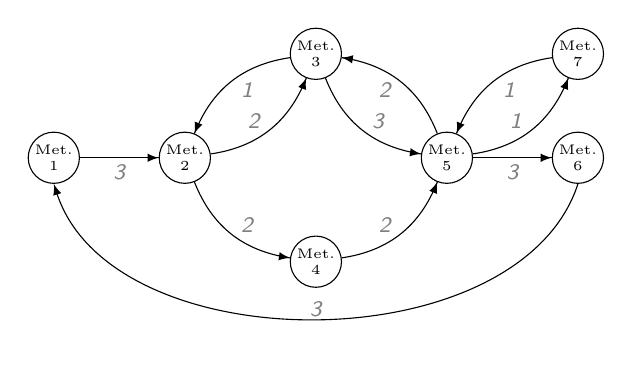
\begin{tikzpicture}[%
  >=latex,
  decoration={%
    markings,
    mark=at position 1.0 with {\arrow{>}}
  },
  every node/.style={%
    font=\sffamily\footnotesize\itshape,
    text=gray,
    text centered,
    align=center
  },
  frame/.style={draw=black,inner sep=2pt}
]

  % Nodes
  \node[lnode,text=black] (A1) {Met.\\1};
  \node[lnode,text=black,right=1.0cm of A1] (A2) {Met.\\2};
  \node[right=1.0cm of A2, lnode,text=black,yshift=1.32cm] (A3) {Met.\\3};
  \node[right=1.0cm of A2, lnode,text=black,yshift=-1.32cm] (A4) {Met.\\4};
  \node[right=1.0cm of A3, lnode,text=black,yshift=-1.32cm] (A5) {Met.\\5};
  \node[right=1.0cm of A5, lnode,text=black] (A6) {Met.\\6};
  \node[right=1.0cm of A5, yshift=1.32cm,lnode,text=black] (A7) {Met.\\7};

  % Intra-node edges
  \draw[postaction={decorate}] (A1) to node [below=0.1pt,yshift=1pt] {3} (A2);
  \draw[postaction={decorate}] (A2) to [bend right=30] node [above left=0.1pt,yshift=-3pt] {2} (A3);
  \draw[postaction={decorate}] (A3) to [bend right=30] node [below right=0.1pt,yshift=3pt] {1} (A2);
  \draw[postaction={decorate}] (A5) to [bend right=30] node [above left=0.1pt,yshift=-3pt] {1} (A7);
  \draw[postaction={decorate}] (A7) to [bend right=30] node [below right=0.1pt,yshift=3pt] {1} (A5);
  \draw[postaction={decorate}] (A3) to [bend right=30] node [above right=0.1pt,yshift=-3pt] {3} (A5);
  \draw[postaction={decorate}] (A5) to [bend right=30] node [below left=0.1pt,yshift=+3pt] {2} (A3);
  \draw[postaction={decorate}] (A2) to [bend right=30] node [above right=0.1pt,yshift=-3pt] {2} (A4);
  \draw[postaction={decorate}] (A4) to [bend right=30] node [above left=0.1pt,yshift=-3pt] {2} (A5);
  \draw[postaction={decorate}] (A5) to node [below=0.1pt,yshift=1pt] {3} (A6);

  % Boundary edges
  \draw[->,postaction={decorate}, bend left=72, distance=2.4cm] (A6.south) to node [above=0.1pt,yshift=-3pt] {3} (A1.south);

\end{tikzpicture}

}\\
      \vspace*{-1.5em}
      \scalebox{0.75}{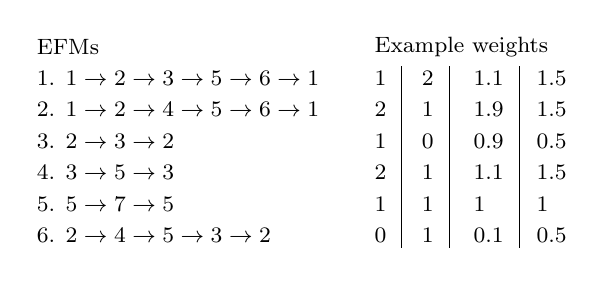
\begin{tikzpicture}[%
    >=latex,
    decoration={%
      markings,
      mark=at position 1.0 with {\arrow{>}}
    },
    every node/.style={%
      font=\sffamily\footnotesize\itshape,
      text=gray,
      text centered,
      align=center
    },
    frame/.style={draw=black,inner sep=2pt}
  ]

  \node[black, font=\rmfamily\footnotesize] (t1) {EFMs};
  \node[black, font=\rmfamily\footnotesize, below=0.4cm of t1.west, anchor=west]
    (t2)
    {1. $1 \rightarrow 2 \rightarrow 3 \rightarrow 5 \rightarrow 6 \rightarrow 1$};
  \node[black, font=\rmfamily\footnotesize, below=0.4cm of t2.west, anchor=west]
    (t3)
    {2. $1 \rightarrow 2 \rightarrow 4 \rightarrow 5 \rightarrow 6 \rightarrow 1$};
  \node[black, font=\rmfamily\footnotesize, below=0.4cm of t3.west, anchor=west]
    (t4)
    {3. $2 \rightarrow 3 \rightarrow 2$};
  \node[black, font=\rmfamily\footnotesize, below=0.4cm of t4.west, anchor=west]
    (t5)
    {4. $3 \rightarrow 5 \rightarrow 3$};
  \node[black, font=\rmfamily\footnotesize, below=0.4cm of t5.west, anchor=west]
    (t6)
    {5. $5 \rightarrow 7 \rightarrow 5$};
  \node[black, font=\rmfamily\footnotesize, below=0.4cm of t6.west, anchor=west]
    (t7)
    {6. $2 \rightarrow 4 \rightarrow 5 \rightarrow 3 \rightarrow 2$};
  \node[black, font=\rmfamily\footnotesize, right=3.25cm of t1] (u1) {Example weights\textcolor{white}{ss}};
  \node[black, font=\rmfamily\footnotesize, below=0.4cm of u1, anchor=south] (u2) {\textcolor{white}{Example weightsss}};
  \node[black, font=\rmfamily\footnotesize, below=0.4cm of u2, anchor=south] (u3) {\textcolor{white}{Example weightsss}};
  \node[black, font=\rmfamily\footnotesize, below=0.4cm of u3, anchor=south] (u4) {\textcolor{white}{Example weightsss}};
  \node[black, font=\rmfamily\footnotesize, below=0.4cm of u4, anchor=south] (u5) {\textcolor{white}{Example weightsss}};
  \node[black, font=\rmfamily\footnotesize, below=0.4cm of u5, anchor=south] (u6) {\textcolor{white}{Example weightsss}};
  \node[black, font=\rmfamily\footnotesize, below=0.4cm of u6, anchor=south] (u7) {\textcolor{white}{Example weightsss}};

  \node[black, font=\rmfamily\footnotesize, below=0.4cm of u1.west, anchor=west,xshift=0cm] (a1) {1};
  \node[black, font=\rmfamily\footnotesize, below=0.4cm of u1.west, anchor=west,xshift=0.6cm] (a2) {2};
  \node[black, font=\rmfamily\footnotesize, below=0.4cm of u1.east, anchor=east,xshift=-0.8cm] (a3) {1.1};
  \node[black, font=\rmfamily\footnotesize, below=0.4cm of u1.east, anchor=east,xshift=0cm] () {1.5};

  \node[black, font=\rmfamily\footnotesize, below=0.4cm of u2.west, anchor=west,xshift=0cm] () {2};
  \node[black, font=\rmfamily\footnotesize, below=0.4cm of u2.west, anchor=west,xshift=0.6cm] () {1};
  \node[black, font=\rmfamily\footnotesize, below=0.4cm of u2.east, anchor=east,xshift=-0.8cm] () {1.9};
  \node[black, font=\rmfamily\footnotesize, below=0.4cm of u2.east, anchor=east,xshift=0cm] () {1.5};

  \node[black, font=\rmfamily\footnotesize, below=0.4cm of u3.west, anchor=west,xshift=0cm] () {1};
  \node[black, font=\rmfamily\footnotesize, below=0.4cm of u3.west, anchor=west,xshift=0.6cm] () {0};
  \node[black, font=\rmfamily\footnotesize, below=0.4cm of u3.east, anchor=east,xshift=-0.8cm] () {0.9};
  \node[black, font=\rmfamily\footnotesize, below=0.4cm of u3.east, anchor=east,xshift=0cm] () {0.5};

  \node[black, font=\rmfamily\footnotesize, below=0.4cm of u4.west, anchor=west,xshift=0cm] () {2};
  \node[black, font=\rmfamily\footnotesize, below=0.4cm of u4.west, anchor=west,xshift=0.6cm] () {1};
  \node[black, font=\rmfamily\footnotesize, below=0.4cm of u4.east, anchor=east,xshift=-0.8cm] () {1.1};
  \node[black, font=\rmfamily\footnotesize, below=0.4cm of u4.east, anchor=east,xshift=0cm] () {1.5};

  \node[black, font=\rmfamily\footnotesize, below=0.4cm of u5.west, anchor=west,xshift=0cm] () {1};
  \node[black, font=\rmfamily\footnotesize, below=0.4cm of u5.west, anchor=west,xshift=0.6cm] () {1};
  \node[black, font=\rmfamily\footnotesize, below=0.4cm of u5.east, anchor=east,xshift=-0.8cm] () {1\textcolor{white}{.0}};
  \node[black, font=\rmfamily\footnotesize, below=0.4cm of u5.east, anchor=east,xshift=0cm] () {1\textcolor{white}{.0}};

  \node[black, font=\rmfamily\footnotesize, below=0.4cm of u6.west, anchor=west,xshift=0cm] (b1) {0};
  \node[black, font=\rmfamily\footnotesize, below=0.4cm of u6.west, anchor=west,xshift=0.6cm] (b2) {1};
  \node[black, font=\rmfamily\footnotesize, below=0.4cm of u6.east, anchor=east,xshift=-0.8cm] (b3) {0.1};
  \node[black, font=\rmfamily\footnotesize, below=0.4cm of u6.east, anchor=east,xshift=0cm] () {0.5};

  % Vertical bars
  \node[black, right=0.1cm of a1, xshift=-1.5mm,yshift=+1.5mm] (l1) {};
  \node[black, right=0.1cm of b1, xshift=-1.5mm,yshift=-1.5mm] (m1) {};
  \draw[black] (l1.center) to (m1.center);
  \node[black, right=0.1cm of a2, xshift=-1.5mm,yshift=+1.5mm] (l2) {};
  \node[black, right=0.1cm of b2, xshift=-1.5mm,yshift=-1.5mm] (m2) {};
  \draw[black] (l2.center) to (m2.center);
  \node[black, right=0.1cm of a3, xshift=-1.5mm,yshift=+1.5mm] (l3) {};
  \node[black, right=0.1cm of b3, xshift=-1.5mm,yshift=-1.5mm] (m3) {};
  \draw[black] (l3.center) to (m3.center);

\end{tikzpicture}
}
    \end{subfigure}
  \end{figure}
\end{document}

